
Section~\ref{sec:codereview} presents the brief history of software inspection and discuss emerging themes from modern code review practices. Subsections from~\ref{sec:reviewtool} to~\ref{sec:inconsistent} discuss various methods that help developers better comprehend software changes, including {\em change decomposition}, {\em refactoring reconstruction}, {\em conflict} and {\em interference} detection, {\em related change search}, and {\em inconsistent change detection}. Section~\ref{sec:differencing} describes various program differencing techniques that serve as a basis for analyzing software changes. Section~\ref{sec:record} describes complementary techniques that record software changes during programming sessions. 

\begin{figure}[ht]
 \centering
 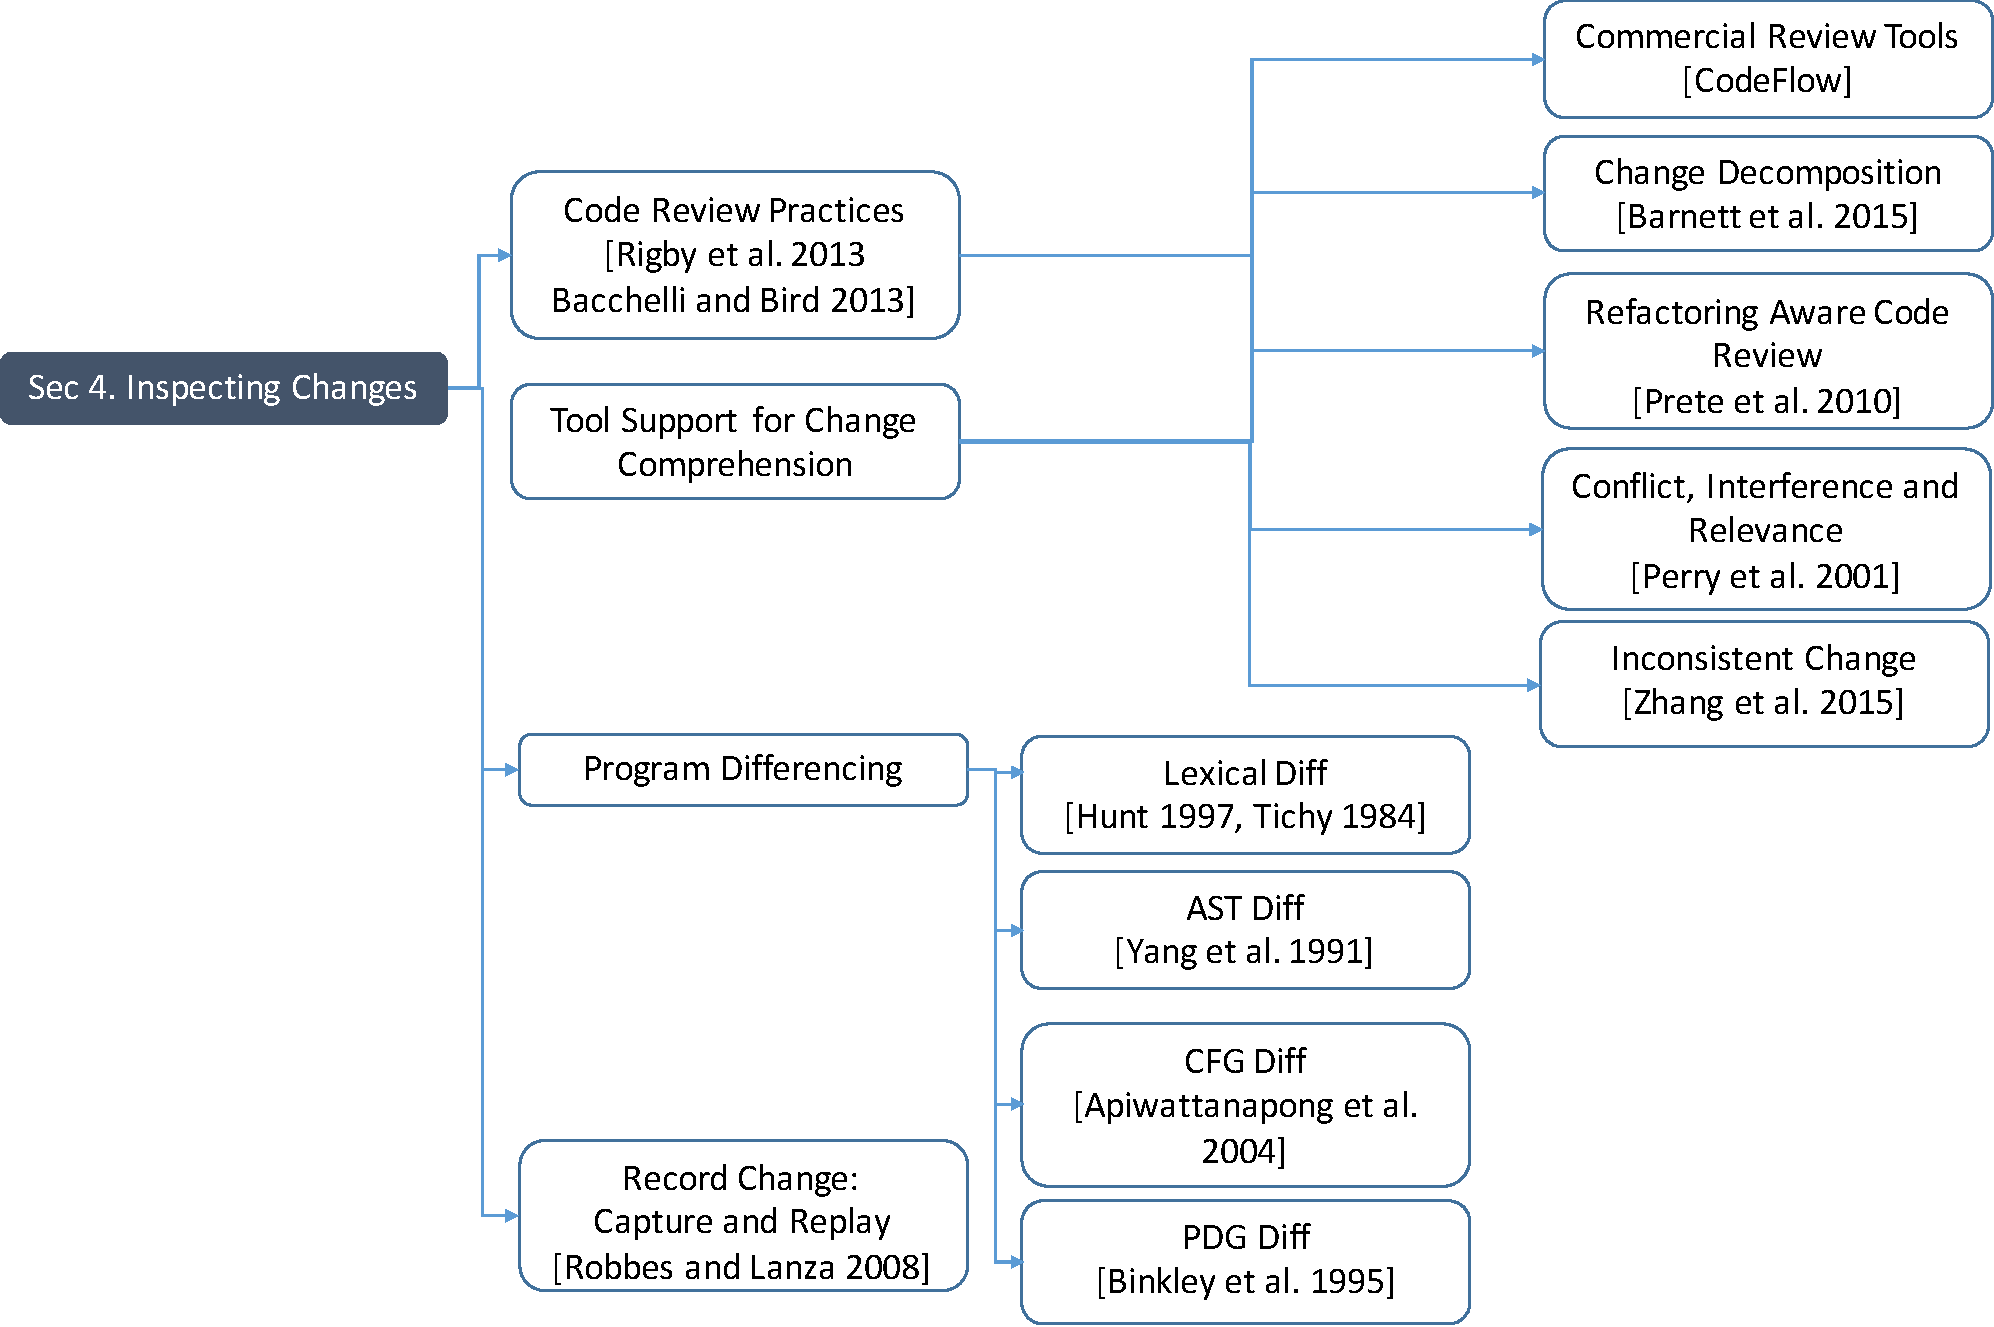
\includegraphics[width=0.95\textwidth]{images/ChangeInspection.pdf}
 \caption{Change Inspection and Related Research Topics} 
 \label{fig:changeinspection} 
\end{figure}

\subsection{Software Inspection and Modern Code Review Practices} 
\label{sec:codereview}

To improve software quality during software evolution, developers often perform {\em code reviews} to manually examine software changes. Michael Fagan from IBM first introduced ``code inspections'', in a seminal paper in 1976~\cite{Fagan1999:checklist}. Code inspections are performed at the end of major software development phases, with the aim of finding overlooked defects before moving to the next phase. Software artifacts are circulated a few days in advance and then reviewed and discussed in a series of meetings. The review meetings include the author of an artifact, other developers to assess the artifact, and a meeting chair to moderate the discussion, and a secretary to record the discussion. Over the years, code inspections have been proven a valuable method to improve software quality. However, the cumbersome and time-consuming nature of this process hinders its universal adoption in practice~\cite{johnson1998reengineering}. 

\begin{figure}[ht]
 \centering
 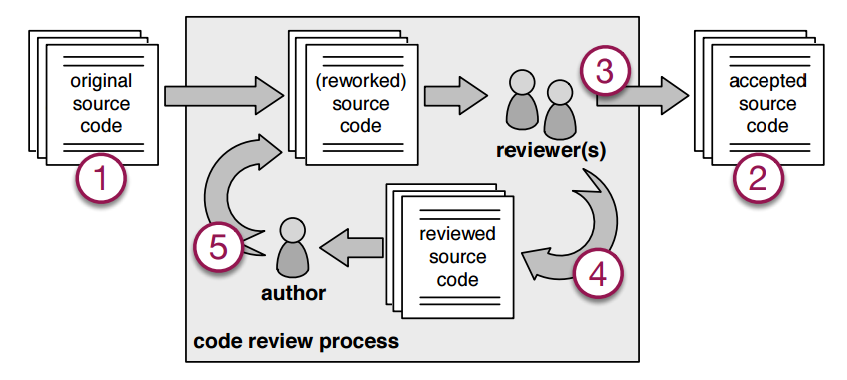
\includegraphics[width=0.75\textwidth]{images/review-process.png}
 \caption{Modern Code Review Process~\cite{beller2014modern}}
 \label{fig:review-process}
\end{figure}

To avoid the inefficiencies in code inspections, most open-source and industrial projects adopt a lightweight, flexible code review process, which we refer to as {\em modern code reviews}. Figure~\ref{fig:review-process} shows the workflow of modern code reviews. The {\em author} first submits the {\em original source code} for review. The {\em reviewers} then decide whether the submitted code meets the quality acceptance criteria. If not, reviewers can annotate the source code with review comments and send back the {\em reviewed source code}. The author then revises the code to address reviewers' comments and send it back for further reviews. This process continues till all reviewers accept the revised code.

In contrast to formal code inspections (Fagan style), modern code reviews occur more regularly and informally on program changes. Rigby et al.~conducted the first case study about modern code review practices in an open-source software (OSS), Apache HTTP server, using archived code review records in email discussions and version control histories~\cite{Rigby2008:apache}. They described modern code reviews as ``early, frequent reviews of small, independent, complete contributions conducted asynchronously by a potentially large, but actually small, group of self-selected experts.'' As code reviews are practiced in software projects with different settings, cultures, and policies, Rigby and Bird further investigated code review practices using a diverse set of open-source and industrial projects~\cite{rigby2013convergent}. Despite differences among projects, they found that many characteristics of modern code reviews have converged to similar values, indicating general principles of modern code review practices. We summarize these convergent code review practices as following.

\begin{itemize}
\item {\it Modern code reviews occur early, quickly, and frequently.} Traditional code inspections happen after finishing a major software component and often last for several weeks. In contrast, modern code reviews happen more frequently and quickly when software changes are committed. For example, the Apache project has review intervals between a few hours to a day. Most reviews are picked up within a few hours among all projects, indicating that reviewers are regularly watching and performing code reviews~\cite{rigby2013convergent}.

\item {\it Modern code reviews often examine small program changes.} During code reviews, the median size of software change varies from 11 to 32 changed lines. The change size is larger in industrial projects, e.g, 44 lines in Android, 78 lines in Chrome, but still much smaller than code inspections, e.g., 263 lines in Lucent. Such small changes facilitate developers to constantly review changes and thus keep up-to-date with the activities of their peers. 
\item {\it Modern code reviews are conducted by a small group of self-selected reviewers.} In OSS projects, no reviews are assigned and developers can select the changes of interest to review. Program changes and review discussions are broadcast to a large group of stakeholders but only a small number of developers periodically participate in code reviews. In industrial projects, reviews are assigned in a mixed manner---the author adds a group of reviewer candidates and individuals from the group then select changes based on their interest and expertise. On average, two reviewers find an optimal number of defects~\cite{rigby2013convergent}.

\item {\it Modern code reviews are often tool-based.} There is a clear trend towards utilizing review tools to support review tasks and communication. Back in 2008, code reviews in OSS projects were often email-based due to a lack of tool support~\cite{Rigby2008:apache}. In 2013 study, some OSS projects and all industrial projects they studied used a review tool~\cite{rigby2013convergent}. More recently, popular OSS hosting services such as GitHub and BitBucket have integrated lightweight review tools to assign reviewers, enter comments, and record discussions. Compared with email-based reviews and traditional software inspections, tool-based reviews provide the benefits of traceability. 

\item {\it Although the initial purpose of code review is to find defects, recent studies find that the practices and actual outcomes are less about finding defects than expected.} A study of code reviews at Microsoft found that only a small portion of review comments were related to defects, which were mainly about small, low-level logical issues~\cite{bacchelli2013expectations}. Rather, code review provides a spectrum of benefits to software teams, such as knowledge transfer, team awareness, and improved solutions with better practices and readability. 

\end{itemize} 

\subsubsection{Commercial Code Review Tools.} 
\label{sec:reviewtool} 

There is a proliferation of review tools, e.g., Phabricator,\footnote{\url{http://phabricator.org}} Gerrit,\footnote{\url{http://code.google.com/p/gerrit/}} CodeFlow,\footnote{\url{http://visualstudioextensions.vlasovstudio.com/2012/01/06/codeflow-code-review-tool-for-visual-studio/}} Crucible,\footnote{\url{https://www.atlassian.com/software/crucible}} and Review Board.\footnote{\url{https://www.reviewboard.org/}} We illustrate CodeFlow, a collaborative code review tool at Microsoft. Other review tools share similar functionality as CodeFlow.

\begin{figure}[ht]
 \centering
 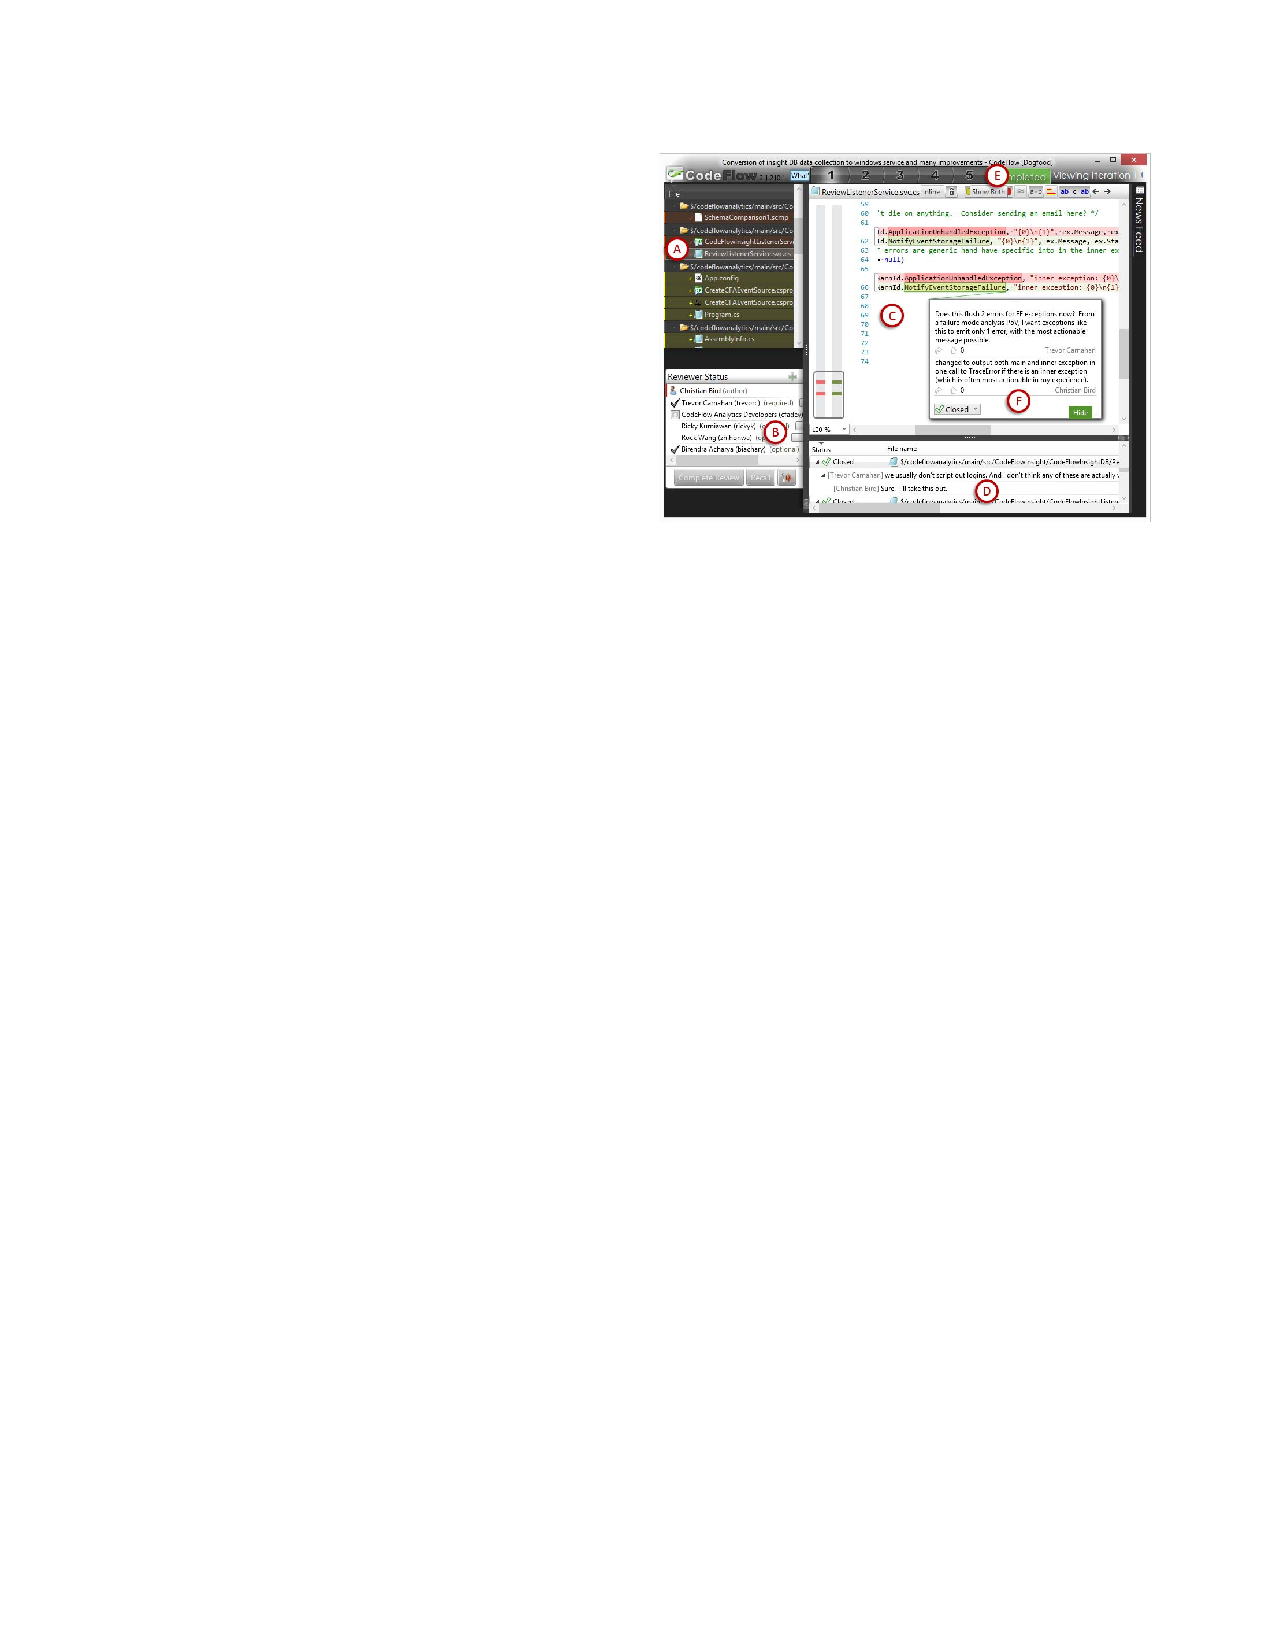
\includegraphics[width=0.75\textwidth]{images/codeflow.pdf}
 \caption{Example of Code Review using CodeFlow~\cite{bosu2015characteristics}}
 \label{fig:codeflow}
\end{figure}

To create a review task, a developer uploads changed files with a short description to CodeFlow. Reviewers are then notified via email and they can examine the software change in CodeFlow. Figure~\ref{fig:codeflow} shows the desktop window of CodeFlow. It includes a list of changed files under review (A), the reviewers and their status (B), the highlighted diff in a changed file (C), a summary of all review comments and their status (D), and the iterations of a review (E). If a reviewer would like to provide feedback, she can select a change and enter a comment which is overlayed with the selected change (F). The author and other reviewers can follow up the discussion by entering comments in the same thread. Typically, after receiving feedback, the author may revise the change accordingly and submit the updated change for additional feedback, which constitutes another review cycle and is termed as an {\em iteration}. In Figure~\ref{fig:codeflow}-E, there are five iterations. CodeFlow assigns a status label to each review comment to keep track of the progress. The initial status is ``Active'' and can be changed to ``Pending'', ``Resolved'', ``Won't Fix'', and ``Closed'' by anyone. Once a reviewer is satisfied with the updated changes, she can indicate this by setting their status to ``Signed Off''. After enough reviewers signed off\textemdash sign-off policies vary by team\textemdash the author can commit the changes to the source repository.

Commercial code review tools facilitate management of code reviews but do not provide deep support for change comprehension. According to Bachhelli et al.~\cite{bacchelli2013expectations}, understanding program changes and their contexts remains a key challenge in modern code review. Many interviewees acknowledged that it is difficult to understand the rationale behind specific changes. All commercial review tools show the highlighted {\em textual, line-level diff} of a changed file. However, when the code changes is distributed across multiple files, developers find it difficult to inspect code changes~\cite{Dunsmore2000:ooinspection}. This obliges reviewers to read changed lines file by file, even when those cross-file changes are done systematically to address the same issue. 
\subsubsection{Change Decomposition.}
\label{sec:decomposition} 

Prior studies also observe that developers often package program changes of multiple tasks to a single code review~\cite{Kawrykow2011,Murphy-Hill2012:refactor,herzig2013impact}. Such large, unrelated changes often lead to difficulty in inspection, since reviewers have to mentally ``untangle'' them to figure out which subset addresses which issue. Reviewers indicated that they can better understand small, cohesive changes rather than large, tangled ones~\cite{Rigby2008:apache}. For example, a code reviewer commented on Gson revision 1154 saying ``{\em I would have preferred to have two different commits: one for adding the new {\ttt getFieldNamingPolicy} method, and another for allowing overriding of primitives.}''\footnote{\url{https://code.google.com/p/google-gson/source/detail?r=1154}} Among change decomposition techniques~\cite{tao2015partitioning,barnett2015helping}, we discuss a representative technique called {\clusterchanges}. 

{\clusterchanges} is a lightweight static analysis technique for decomposing large changes~\cite{barnett2015helping}. The insight is that program changes that address the same issue can be related via implicit dependency such as {\em def-use} relationship. For example, if a method definition is changed in one location and its call-sites are changed in two other locations, these three changes are likely to be related and should be reviewed together. Given a code review task, {\clusterchanges} first collects the set of definitions for types, fields, methods, and local variables in the corresponding project under review. Then {\clusterchanges} scans the project for all uses (i.e., references to a definition) of the defined code elements. For instance, any occurrence of a type, field, or method either inside a method or a field initialization is considered to be a use. Based on the extracted def-use information, {\clusterchanges} identifies three relationships between program changes. 

\begin{itemize}
	\item {\bf Def-use relation}. If the definition of a method or a field is changed, all the uses should also be updated. The change in the definition and the corresponding changes in its references are considered related.
	\item {\bf Use-use relation}. If two or more uses of a method or a field defined within the change-set are changed, these changes are considered related. 
	\item  {\bf Enclosing relation}. Program changes in the same method are considered related, under the assumption that  (1) program changes to the same method are often related, and (2) reviewers often inspect methods atomically rather than reviewing different changed regions in the same method separately.
\end{itemize} 

Given these relations, {\clusterchanges} creates a partition over the set of program changes by computing a transitive closure of related changes. On the other hand, if a change is not related to any other changes, it will be put into a specific partition, {\em miscellaneous changes}.


\subsubsection{Refactoring Aware Code Review.}  
\label{sec:refactoringreview} 

Identifying which refactorings happened between two program versions is an important research problem, because inferred refactorings can help developers understand software modifications made by other developers during peer code reviews. Reconstructed refactorings can be used to update client applications that are broken due to refactorings in library components. Furthermore, they can be used to study the effect of refactorings on software quality empirically when the documentation about past refactorings is unavailable in software project histories. 

{\bf Refactoring reconstruction} techniques compare the old and new program versions and identify corresponding entities based on their {name similarity} and {structure similarity}\cite{Demeyer2000, Zou2005, Malpohl2000, Dig2006, Weissgerber2006}. Then based on how basic entities and relations changed from one version to the next, concrete refactoring type and locations are inferred. For example, Xing et al.'s approach~\cite{UMLDiff2005} UMLDiff extracts class models from two versions of a program, traverses the two models, and identifies corresponding entities based on their {name similarity} and {structure similarity} {(i.e., similarity in type declaration and uses, field accesses, and method calls)}. Xing {et al.} later presented an extended approach to refactoring reconstruction based on change-facts {\em queries}~\cite{Eleni01}. They first extract facts regarding design-level entities and relations from each individual source code version. These facts are then pairwise compared to determine how the basic entities and relations have changed from one version to the next. Finally, queries corresponding to well-known refactoring types are applied to the change-facts database to find concrete refactoring instances. Among these refactoring reconstruction techniques, we introduce a representative example of refactoring reconstruction, called RefFinder in details~\cite{Prete2010:reffinder,Kim2010:reffinder}.   

% Demeyer {et al.} first proposed the idea of inferring refactorings from two program versions by comparing two program versions. They used a set of ten characteristic metrics, such as LOC and the number of method calls within a method~\cite{Demeyer2000}. Zou and Godfrey first coined the term origin analysis, which serves as a basis for refactoring reconstruction by matching code elements using multiple criteria (e.g., names, signatures, metric values, callers, and callees)~\cite{Zou2005}. Their approach infers merge, split, and rename refactorings. Van Rysselberghe and Demeyer used a clone detector to detect moved methods~\cite{Rysselberghe2003}.  Antoniol {et al.} identified class-level refactorings using a vector space information retrieval approach~\cite{Antoniol2004}. Malpohl {et al.} \cite{Malpohl2000} align tokens using {\it diff} and infers a function or variable renaming when distinct tokens are surrounded by mapped token pairs. Dig et al.'s approach, {Refactoring Crawler} identifies refactorings in two stages~\cite{Dig2006}. First, it finds a list of code element pairs using {\em shingles} (a metric-based fingerprint) and performs a semantic analysis based on reference relationships (calls, instantiations, uses of types, import statements). The second part of the algorithm is an iterative, fix point algorithm that considers refactorings in a top-down order. 

%Wei{\ss}gerber and Diehl's approach~\cite{Weissgerber2006} extracts added and deleted entities (fields, methods, and classes) by parsing deltas from a version control system and then compares these entities based on their {name similarity}. When it cannot disambiguate all refactoring candidates, it uses a {clone detector} (CCFinder~\cite{Kamiya2002}) to rank these candidates. S. Kim et al.'s approach~\cite{SKim2005} considers various information (such as {calling relationships}, {clone detection} results, and {name similarity}) to match method-headers.  Wu et al.'s approach~\cite{Wu2010:AHA} is a hybrid approach that combines the strengths of {call-graph matching} and {name-similarity} based matching. Nguyen et al.'s approach~\cite{Nguyen2010:GAA} identifies refactorings in libraries to support adaptation of the client applications that use those libraries. Similar to Xing et al.'s approach, the algorithm matches code elements top-down based on method name similarity and method body contents. Fluri et al.'s approach~\cite{FWP2007} compares two versions of abstract syntax trees, computes tree-edit operations, and maps each tree-edit to atomic AST-level change types (e.g., parameter ordering change).

\label{sec:intro} 
\begin{figure*}
\centering
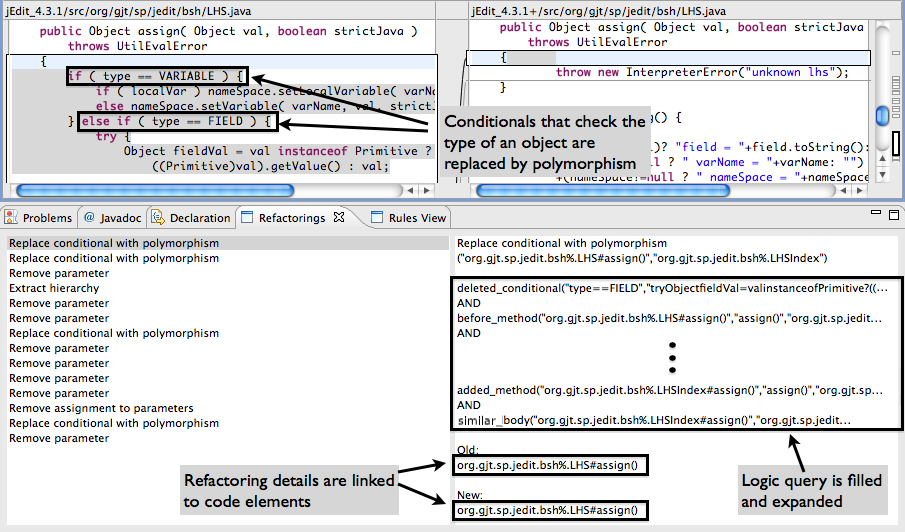
\includegraphics[width=0.95\textwidth]{images/reffinder.png}
\caption{RefFinder infers a {\it replace conditionals with polymorphism} refactoring from change facts {\it deleted\_conditional}, {\it after\_subtype}, {\it before\_method}, {\it added\_method} and {\it similar\_body}.\cite{Kim2010:reffinder}}
 \label{fig:reffinderscreenshot}
\end{figure*}

\paragraph{Example: RefFinder.}

{\em RefFinder} is a logic-query based approach for inferring various types of refactorings in Fowler's catalog~\cite{Prete2010:reffinder}. It first encodes each refactoring type as a structural constraint on the program before and after the refactoring in a template logic rule. It then compares the syntax tree of each version to compute change facts such as {\tt added\-\_subtype}, at the level of code elements (packages, types, methods, and fields), structural dependencies (subtyping, overriding, method-calls, and field-accesses), and control constructs (while, if-statements, and try-catch blocks). It determines a refactoring inference order to find atomic refactorings before composite refactorings. 

For example, consider an \emph{extract superclass} refactoring that extracts common functionality in different classes into a superclass. It finds each {\it pull-up-method} refactoring and then tests if they combine to an \emph{extract superclass} refactoring. For each refactoring rule, it converts the antecedent of the rule to a logic query and invokes the query on the change-fact database. If the query returns the constant bindings for logic variables, it creates a new logic fact for the found refactoring instance and {\em writes} it to the fact-base. For example, by invoking a query {\tt pull\-\_up\_method\-(?method, ?class, ?superclass) $\wedge$ added\_type\-(?superclass)}, it finds a concrete instance of {\it extract superclass} refactoring. Figure~\ref{fig:complexrefactoring} illustrates an example refactoring reconstruction process. 

\begin{figure}
\scriptsize
%\centering 
\begin{tabular}{|p{0.17\textwidth}|p{0.83\textwidth}|}
\hline
{pull\_up\_method} & You have methods with identical results on subclasses; move them to the superclass. \\
\hline
template &
\factfont{deleted\_method(m1, n, t1) $\wedge$ after\_subtype(t2, t1) $\wedge$ added\_method(m1, n, t2) $\Rightarrow$ pull\_up\_method(n, t1, t2)}  \\
\cline{1-2}
logic rules&  \factfont{pull\_up\_method(m1, t1, t2) $\wedge$ added\_type(t2) $\Rightarrow$ extract\_superclass(t1,t2)} \\
\hline
code example & \vspace{-5mm} 
\begin{verbatim} 
+public class Customer{ 
+   chargeFor(start:Date, end:Date) { ... } ...}  
-public class RegularCustomer{
+public class RegularCustomer extends Customer{
-   chargeFor(start:Date, end:Date){ ... } ...}
+public class PreferredCustomer extends Customer{ 
- chargeFor(start:Date, end:Date){ ... } // deleted ... } 
\end{verbatim} 
\vspace{-5mm}
\\ \hline
found &
\factfont{pull\_up\_method("chargeFor", "RegularCustomer", "Customer")} \\

refactorings& \factfont{pull\_up\_method("chargeFor", "PreferredCustomer", "Customer")}  \\
& \factfont{extract\_superclass("RegularCustomer", "Customer")} \\
& \factfont{extract\_superclass("PreferredCustomer", "Customer")}\\
\hline
\end{tabular}
\caption{Reconstruction of \emph{Extract Superclass} Refactoring} 
\label{fig:complexrefactoring}
\end{figure} 

This approach has two advantages over other approaches. First, it analyzes the body of methods including changes to the control structure within method bodies. Thus, it can handle the detection of refactorings such as {\it replacing conditional code with polymorphism}. Second, it handles composite refactorings, since the approach reasons about which constituent refactorings must be detected first and reason about how those constituent refactorigs are knit together to detect higher-level, composite refactorings. It supports 63 out of 72 refactoring types in Fowler's catalog. As shown in Figure \ref{fig:reffinderscreenshot}, RefFinder visualizes the reconstructed refactorings as a list.  The panel on the right summarizes key details of the selected refactoring and allows the developer quickly navigate to the associated code fragments. 

\subsubsection{Change Conflicts, Interference, and Relevance. } 
\label{sec:conflict} 
As development teams become distributed, and the size of the system is often too large to be handled by a few developers, multiple developers often work on the same module at the same time. In addition, the market-pressure to develop new features or products makes parallel development no longer an option.  A study on a subsystem of Lucent 5ESS telephone found that 12.5\% of all changes are made by different developers to the same files within 24 hours, showing a high degree of parallel updates~\cite{Perry2001:parallel}. A subsequent study found that even though only 3\% of the changes made within 24 hours by different developers physically overlapped each other's changes at a textual level but there was a high degree of semantic interference among parallel changes at a data flow analysis level (about 43\% of revisions made within one week). They also discovered a significant correlation between files with a high degree of parallel development and the number of defects~\cite{Shao2007:interference}. 

Most version control systems are only able to detect most simple types of conflicting changes\textemdash changes made on top of other changes~\cite{mens:survey02}. To detect changes that indirectly conflict with each other, some define the notion of {\em semantic interference} using program slicing on program dependence graphs, and integrate non-interfering versions only if there is no overlap between program slices~\cite{Horwitz1989}. As another example, some define semantic interference as the overlap between the data-dependence based impact sets of parallel updates~\cite{Shao2007:interference}. 

%Several techniques identify related changes across revisions rely on temporal proximity \cite{Bevan2005, Fischer2003, German2004:softchange, Zimmermann2004b}, syntactic dependence \cite{Chesley2005}, physical location \cite{Zeller1999}, committer information \cite{Fischer2003, German2004:softchange, Zimmermann2004b}, history of co-changes \cite{Gall1998, Ying2004, Zimmermann2004}, and content similarity~\cite{Kim:2009,NNP2009}. For example, Crisp \cite{Chesley2005} computes atomic structural changes such as method additions and deletions via AST differencing and groups syntactically dependent changes through def-use relationships.  
%\subsubsection{Search of Software Changes.}
%\label{sec:changesearch} 

%SCM query systems such as SCQL \cite{Hindle2005} or CVS Query \cite{bonsai} can search check-ins based on who changed which file and when, but cannot search change history by code elements and dependencies. Systems such as Hipikat \cite{Hipikat}, Bridge \cite{Venolia2006:bridge}, Tesseract \cite{Tesseract}, and Deep Intellisense \cite{Holmes2008:intellisense} automatically associate different types of software artifacts (e.g., check-ins, bug reports, and emails) but provide limited help in querying code changes. 

%Several visualization tools focus on representing changes between versions \cite{Ball1996,Eick2002,Girba2004,Holt1996,Lanza01:sv,Lanza2003,Rysselberghe2004a}. For example, Evolution Matrix \cite{Lanza01:sv} visualizes classes that have been added, modified, and deleted in different versions and creates a 2-D matrix where the rows represent classes and the columns represent the versions of the artifact. These tools generally require substantial interpretation effort by developers to understand system evolution. Studying program evolution by analyzing existing software project artifacts is increasingly becoming a popular research approach. Existing research infrastructures for mining software artifacts focus on data extraction \cite{Bevan2005,Fischer2003} and integration of different types of software artifacts \cite{Hipikat, Venolia2006:bridge,Tesseract, Begel2010:codebook}. 

\subsubsection{Detecting and Preventing Inconsistent Changes to Clones.} 
\label{sec:inconsistent} 

Code cloning is an important source of bugs in operating systems~\cite{releasenote}. In 65\% of the ported code, at least one identifier is renamed, and in 27\% cases at least one statement is inserted, modified, or deleted~\cite{Li2004:CP-Miner}. An incorrect adaptation of ported code often leads to porting errors~\cite{Jiang2007}. Interviews with developers confirm that inconsistencies in clones are indeed bugs and report that {\em ``nearly every second, unintentional inconsistent changes to clones lead to a fault."}~\cite{Juergens2009:clone-bug}.  Several techniques find inconsistent changes to similar code fragments by tracking copy-paste code and by comparing the corresponding code and its surrounding contexts~\cite{Li2004:CP-Miner, Jablonski2007:CReN, Ray2013:spa, Jiang2007, Jiang2007a}.  Below, we present a representative technique, called {\critics}. 
%For example, SPA detects a broader scope of inconsistent renamings by tokenizing function names, file names, and identifier names using a camel case naming convention and mapping corresponding tokens. Our algorithm detects an inconsistency when a token in one context maps to multiple tokens in the other context.  For example, when code is ported from~\texttt{Export.java} to~\texttt{Import.java}, SPA checks whether all names related to~\texttt{export} are updated to~\texttt{import}.  ~\cite{Ray2013:spa} 

% Jiang et al.~show that an inconsistent context can also cause porting errors~\cite{Jiang2007}. However, their definition of context is limited to the {\em innermost} control flow construct surrounding the cloned code. They identify syntactic clones using AST level similarity~\cite{Jiang2007a}, and then detect inconsistencies by comparing the contexts. 
%DejaVu extends the work by Jiang et al. by using several filtering heuristics, such as assessing textual similarity and pruning non-cloned contexts, to improve its precision~\cite{Gabel2010:dejavu}. 

%\begin{figure}[ht]
% \centering
% 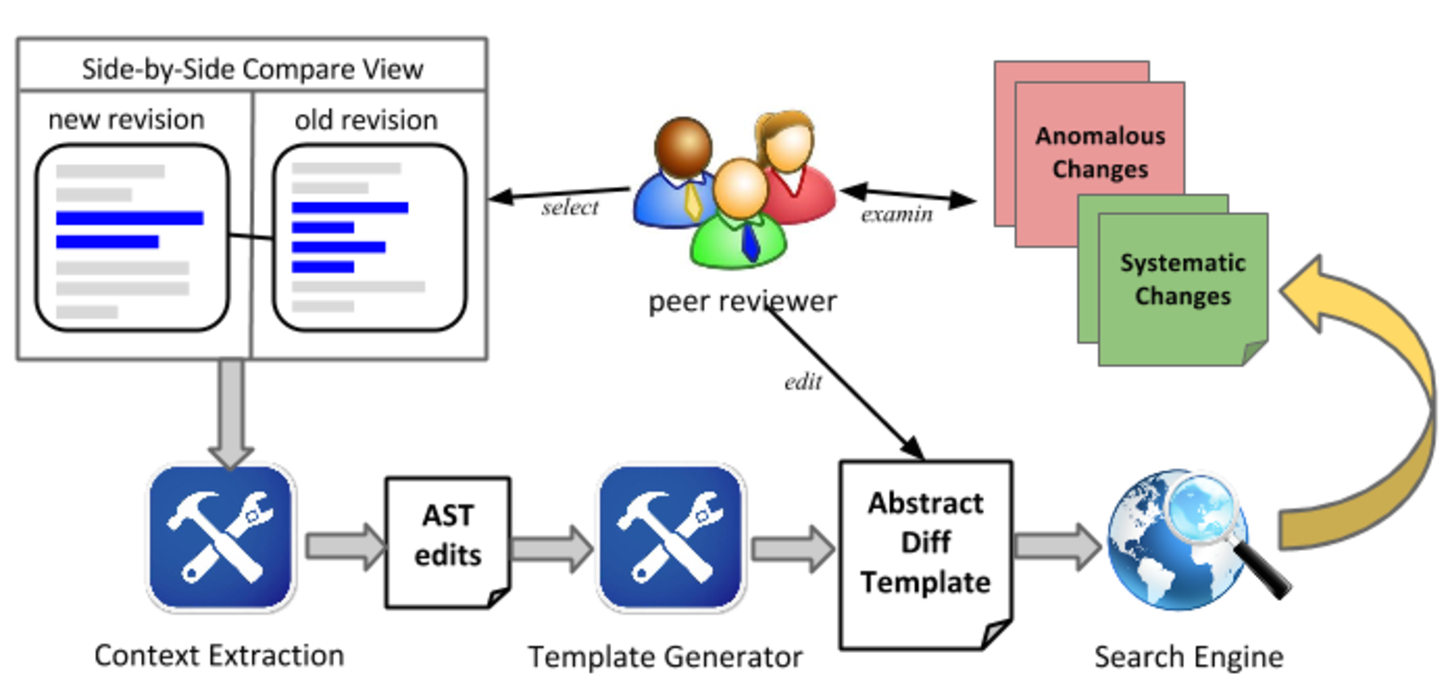
\includegraphics[width=0.8\textwidth]{images/critics-workflow.pdf}
% \caption{The workflow of {\critics}}
% \label{fig:critics-workflow}
%\end{figure}

\paragraph{Example: {\critics}.} {\critics} allows reviewers to interactively detect inconsistent changes through template-based code search and anomaly detection~\cite{zhang2015interactive}. Given a specified change that a reviewer would like to inspect, {\critics} creates a change template from the selected change, which serves as the pattern for searching similar changes. {\critics} includes {\em change context} in the template---unchanged, surrounding program statements that are relevant to the selected change. {\critics} models the template as Abstract Syntax Tree (AST) edits and allows reviewers to iteratively customize the template by parameterizing its content and by excluding certain statements. {\critics} then matches the customized template against the rest of the codebase to summarize similar changes and locate potential inconsistent or missing changes. Reviewers can incrementally refine the template and progressively search for similar changes until they are satisfied with the inspection results. This interactive feature allows reviewers with little knowledge of a codebase to flexibly explore the program changes with a desired pattern. %Figure~\ref{fig:critics-workflow} describes the interactive workflow of {\critics}. 

\begin{figure}[ht]
 \centering
 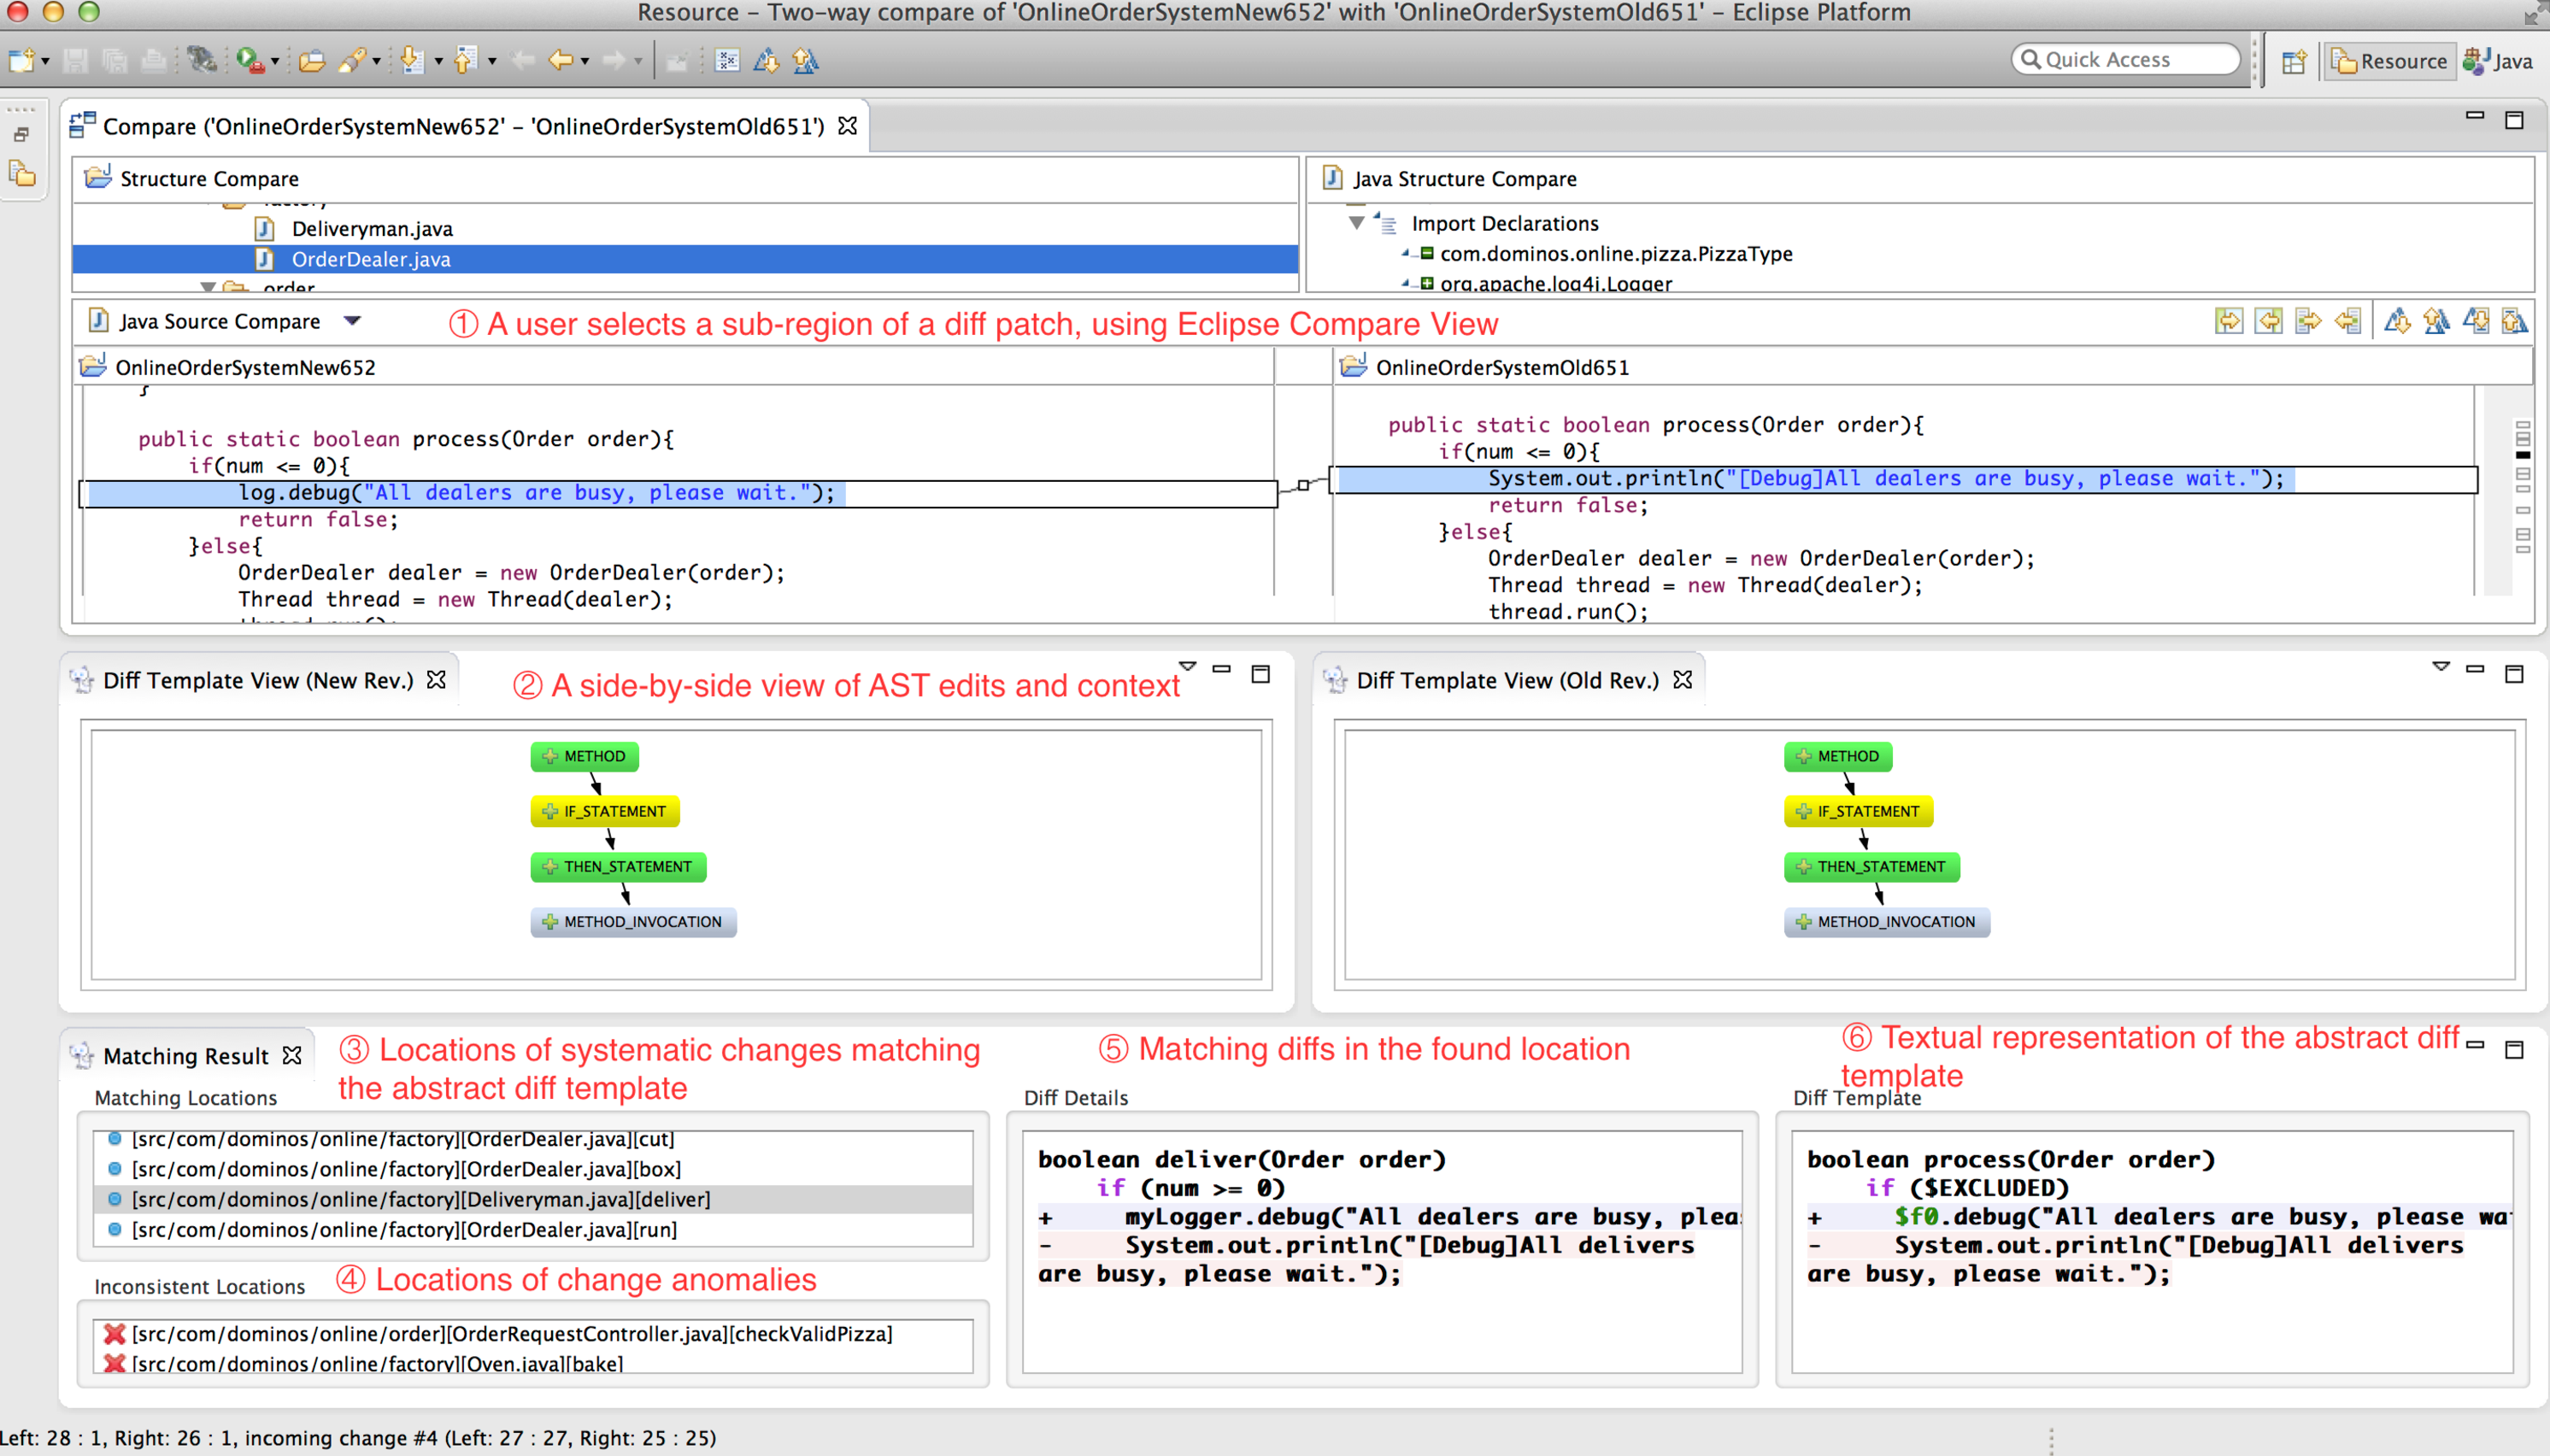
\includegraphics[width=\textwidth]{images/critics-UI.pdf}
 \caption{A screen snapshot of {\critics}'s Eclipse plugin and its features}
 \label{fig:critics-UI}
\end{figure}

Figure~\ref{fig:critics-UI} shows a screenshot of {\critics} plugin. {\critics} is integrated with the {Compare View} in Eclipse, which displays line-level differences per file (see \ding{172} in Figure~\ref{fig:critics-UI}). A user can specify a program change she wants to inspect by selecting the corresponding code region in the Eclipse Compare View. The {Diff Template View} (see \ding{173} in Figure~\ref{fig:critics-UI}) visualizes the change template of the selected change in a side-by-side view. Reviewers can parameterize concrete identifiers and exclude certain program statements by clicking on the corresponding node in the Diff Template View. {Textual Diff Template View} (see \ding{177} in Figure~\ref{fig:critics-UI}) shows the change template in a unified format. The {Matching Result View} summarizes the consistent changes as {\em similar changes} (see \ding{174} in Figure~\ref{fig:critics-UI}) and inconsistent ones as {\em anomalies} (see \ding{175} in Figure~\ref{fig:critics-UI}).
